%%%%%%%%%%%%
%
% $Autor: Wings $
% $Datum: 2019-03-05 08:03:15Z $
% $Pfad: TemplateSensor $
% $Version: 4250 $
% !TeX spellcheck = en_GB/de_DE
% !TeX encoding = utf8
% !TeX root = filename 
% !TeX TXS-program:bibliography = txs:///biber
%
%%%%%%%%%%%%
\chapter{Backend-Architektur im LoRaWAN-System}
	Dieses Kapitel beschreibt die Backend-Architektur eines \ac{lorawan}-Systems und erläutert die Zusammenarbeit von \acf{lns}, \acf{as} und \acf{js}. Darüber hinaus werden die Interaktionen der Komponenten im Uplink- und Downlink-Prozess dargestellt sowie zentrale Unterschiede zwischen öffentlichen und privaten \acs{lorawan}-Netzen diskutiert.
	
\section{Übersicht der Backend-Komponenten}
	\begin{figure}[H]
		\centering
		\resizebox{\textwidth}{!}{
			\begin{tikzpicture}
				\LoRaWANBAckendinfrastructure
			\end{tikzpicture}
		}
		\caption{\ac{lorawan} Backend-Architektur \cite{Montagny:2022}}
	\end{figure}

\section{\acl{lns} \label{server:lns}}
	Der Netzwerkserver verwaltet das gesamte \ac{lorawan}-Netzwerk. Er verarbeitet die von den Gateways 	empfangenen, verschlüsselten Nachrichten, entfernt doppelte Pakete und gewährleistet eine sichere Übertragung durch die Verwendung von AES-128-Verschlüsselung. Dies gilt sowohl für Uplink-Nachrichten (vom Endgerät zum \ac{lns}) als auch für Downlink-Nachrichten (vom \ac{lns} zum Endgerät). Der \ac{lns} stellt sicher, dass alle Geräte im Netzwerk authentifiziert sind und die Integrität jeder Nachricht gewahrt bleibt. Dabei hat der Netzwerkserver keinen Zugriff auf den eigentlichen Anwendungsinhalt der Daten. Zudem ist der Netzwerkserver für die Anpassung des Spreading Factors und der Datenrate, das Scheduling von Downlink-Nachrichten sowie die Weiterleitung der Nachrichten an die Anwendungsserver verantwortlich \cite{Semtech:2024, Montagny:2022}.

	Der \ac{lns} bildet die zentrale logische Instanz im \ac{lorawan}-System. Er implementiert die vollständige MAC-Schichtlogik, verwaltet die Kommunikation mit allen Endgeräten und koordiniert das gesamte \ac{lorawan}-Netzwerk. Für den Betrieb ist mindestens ein Gateway erforderlich, das die Funkpakete der Endgeräte empfängt und an den \ac{lns} weiterleitet. Zusätzlich wird ein Anwendungserver benötigt, der die Nutzdaten entschlüsselt. In grö{\ss}eren oder skalierenden Netzwerken kommt ein dedizierter Join Server hinzu, der die Authentifizierung der Endgeräte übernimmt und die Sitzungsschlüssel generiert \cite{Semtech:2024, Montagny:2022}.
	
\subsection{Kernaufgaben des Network Servers}
\subsubsection{Deduplication eingehender Frames}
	Wenn ein Uplink-Frame von mehreren Gateways empfangen wird, werden alle Kopien über das Backhaul an den Netzwerkserver übertragen. \textcite{LoRaAlliance:2020c} weist darauf hin, dass in diesem Fall eine Deduplikation durchgeführt werden muss, sodass nur eine logische Nachricht an den \ac{as} weitergereicht wird. Ein konkreter Algorithmus ist jedoch nicht Teil der Spezifikation und wird den jeweiligen Implementierungen der \ac{lns}-Anbieter überlassen.

	Ein praktisches Beispiel für einen solchen Mechanismus liefert The Things Network (TTN). In der technischen Dokumentation beschreibt TTN, dass eingehende Uplink-Nachrichten während eines kurzen Zeitfensters gesammelt und anhand eines Hash-Werts (MD5 über den Payload) identifiziert werden. Da der Payload bei allen Duplikaten identisch ist, besitzen diese Frames denselben Hash und können somit zuverlässig zusammengeführt werden. Während der Deduplikationsphase, die typischerweise etwa 200\,ms beträgt, werden zusätzliche Metadaten wie RSSI, SNR und Gateway-Identifikatoren aggregiert. Auf diese Weise entsteht ein einziges, konsolidiertes Uplink-Paket, das anschlie{\ss}end an den \ac{as} übermittelt wird, während redundante Kopien verworfen oder ausschlie{\ss}lich für Metadatenanalyse verwendet werden. Dieser Ansatz erlaubt es zudem, aus den unterschiedlichen Empfangsparametern geeignete Gateways für potenzielle Downlink-Übertragungen auszuwählen \cite{TTN:2021}.

\subsubsection{MIC-Prüfung und Sicherheitsvalidierung}
	Um ein eingehendes Paket authentifizieren zu können, berechnet der \ac{lns} den \PYTHON{MIC} anhand des \PYTHON{NwkSKey} über alle Felder des empfangenen \textbf{MAC Payload} - Frames neu. 

	\begin{figure}[H]
		\centering
		\begin{tikzpicture}
			\micComparison
		\end{tikzpicture}
		\caption{Schematische Darstellung der \PYTHON{MIC}-Verifizierung \cite{Montagny:2022}}
	\end{figure}
	
	Anschlie{\ss}end wird dieser berechnete Wert mit dem im Frame enthaltenen \PYTHON{MIC}-Feld verglichen.
	
	\begin{figure}[H]
		\centering
		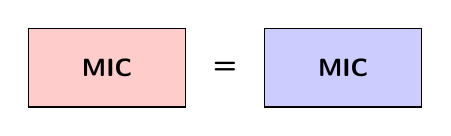
\begin{tikzpicture}
			\filldraw[fill=red!20] (0, 0) rectangle (2, 1);
			\filldraw[fill=blue!20] (3, 0) rectangle (5, 1);
			\node[font=\sffamily] at (2.5, 0.5) {\textbf{=}};
			\node[font=\sffamily\small] at (1, 0.5) {\textbf{MIC}};
			\node[font=\sffamily\small] at (4, 0.5) {\textbf{MIC}};
		\end{tikzpicture}
		\caption{Vergleich der \PYTHON{MIC} - Nummern\cite{Montagny:2022}}
	\end{figure}
	
	 Stimmen beide Werte überein, kann der Server sicherstellen, dass die Nachricht tatsächlich zu diesem Netzwerk gehört und während der Übertragung nicht manipuliert wurde. Nur ein Frame mit gültiger \PYTHON{MIC}-Prüfung wird weiterverarbeitet.

	
\subsubsection{Verwaltung der Frame Counter (\PYTHON{FCntUp}/\PYTHON{FCntDown})}
	Die Verwaltung der Frame Counter ist ein zentraler Bestandteil der Sicherheitsmechanismen von \ac{lorawan}. Jeder Uplink-Frame eines Endgeräts wird mit einem monoton steigenden Zähler \PYTHON{FCntUp} versehen, der sicherstellt, dass Nachrichten weder wiederholt noch in veränderter Reihenfolge akzeptiert werden. Der \ac{lns} führt für jedes Endgerät eine eigene Zählerverwaltung und verwirft jeden Uplink, dessen \PYTHON{FCntUp}-Wert nicht strikt grö{\ss}er als der zuletzt gespeicherte Wert ist. Dadurch wird ein wirkungsvoller Schutz gegen Replay-Angriffe erreicht.

	Analog dazu verwaltet der \ac{lns} den Downlink-Zähler \PYTHON{FCntDown}, der von ihm selbst generiert und vom Endgerät bei jedem empfangenen Downlink überprüft wird. Auch dieser Wert muss monoton ansteigen, da das Endgerät sonst die Nachricht verwertet. Die Konsistenz beider Zähler ist somit Voraussetzung für eine korrekte Entschlüsselung der Frames und die erfolgreiche Überprüfung des \ac{mic}. Eine fehlerhafte oder inkonsistente Zählerverwaltung führt unmittelbar zur Ungültigkeit der Nachricht und verhindert deren weitere Verarbeitung im Netzwerk \cite{Montagny:2022} \cite{LoRaAlliance:2020b} \cite{LoRaAlliance:2020c}.

\subsubsection{Weiterleitung der Applikationsdaten}
	Nach erfolgreicher \ac{mic}-Prüfung und Validierung des Frame Counters übergibt der \ac{lns} den entschlüsselten \PYTHON{FRMPayload} jedoch nicht an die Netzlogik, sondern leitet ihn gemä{\ss} dem Ende-zu-Ende-Sicherheitsmodell direkt an den \ac{as} weiter. Da der \ac{lns} keinen Zugriff auf den \ac{appskey} besitzt, kann er die Anwendungsdaten weder einsehen noch modifizieren. Seine Aufgabe beschränkt sich darauf, die für den Netzwerkbetrieb relevanten Felder wie MAC-Befehle, Frame Counter oder Empfangsmetadaten zu verarbeiten und die Nutzlast anschlie{\ss}end transparent weiterzuleiten.

	Der \ac{as} entschlüsselt den  \PYTHON{FRMPayload} mithilfe des \ac{appskey} und führt dort die eigentliche Applikationslogik aus. Gleichzeitig kann der \ac{as} Downlink-Daten generieren, die wiederum über den \ac{lns} an das Endgerät übermittelt werden  \cite{Montagny:2022} \cite{LoRaAlliance:2020b} \cite{LoRaAlliance:2020c}.


\subsection{\acl{adr} \acs{adr}}
	LoRaWAN ermöglicht es Endgeräten, ihre Datenrate sowie die Sendeleistung individuell an die Funkbedingungen anzupassen. Dieser Mechanismus wird vom Netzwerk genutzt, um die Anzahl der Wiederholungen, die Datenrate und die Sendeleistung eines Endgeräts dynamisch zu steuern. Das Verfahren wird als \acl{adr} (\acs{adr}) bezeichnet und hat zum Ziel, die höchstmögliche stabile Datenrate bei minimaler Sendeleistung zu erreichen \cite{LoRaAlliance:2020b, Montagny:2022}.
	
	Der \ac{lns} bestimmt die optimale Datenrate, indem er die übermittelten Link-Metriken analysiert und eine Konfiguration auswählt, die sowohl Energieeffizienz als auch Übertragungssicherheit maximiert. Bei stabilen Funkbedingungen erhöht der \ac{lns} schrittweise die Datenrate und reduziert die Sendeleistung. Verschlechtern sich die Bedingungen oder bleiben Downlinks aus, wird wieder auf robustere Einstellungen zurückgeschaltet \cite{Montagny:2022, LoRaAlliance:2020b}. 
	
	Nach einem Neustart senden Endgeräte zunächst mit maximaler \PYTHON{TXPower} und der niedrigsten Datenrate, bis der \ac{lns} ihnen über das MAC-Kommando \PYTHON{LinkADRReq} eine neue Konfiguration zuweist \cite{LoRaAlliance:2020b}. 

	Die LoRaWAN-Spezifikation definiert keinen festen ADR-Algorithmus. Sie legt lediglich fest, dass ein \ac{lns} über \texttt{LinkADRReq}-Kommandos Parameter wie Datenrate, Sendeleistung und Wiederholungsrate ändern darf. Die konkrete Entscheidungslogik – also wann und wie diese Parameter angepasst werden – bleibt vollständig implementierungsspezifisch.

\subsubsection{Beispiel eines \ac{adr}-Algorithmus nach Semtech}
	
	\textcite{Semtech:2016} beschreibt in \citetitle{Semtech:2016} einen vollständigen \ac{adr}-Algorithmus, 
	der auf den letzten 20 Uplink-Frames eines Endgeräts basiert. Für jeden empfangenen Uplink ermittelt der Netzwerkserver den jeweils höchsten der von den verschiedenen Gateways gemessenen SNR-Werte (\(SNR_{max}\)). Die letzten zwanzig Werte von \(SNR_{max}\), die zugehörigen Frame Counter sowie die Anzahl der empfangenden Gateways werden in einer gleitenden Tabelle gespeichert, in der ältere Einträge fortlaufend überschrieben werden.
	
	\begin{table}[H]
		\centering
		\begin{tabular}{|c|c|c|}
			\hline
			\textbf{\PYTHON{FCnt}} & \textbf{\(SNR_{max}\) [dB]} & \textbf{Gateway-Anzahl} \\
			\hline
			10 & -6  & 2 \\
			\hline
			11 & -7  & 2 \\
			\hline
			12 & -25 & 1 \\
			\hline
			14 & -25 & 2 \\
			\hline
			\textit{usw.} & & \\
			\hline
			29 & -7  & 2 \\
			\hline
		\end{tabular}
		\caption{Beispielhafte SNR-Empfangswerte für ein Endgerät}
	\end{table}
	
	Zur Bestimmung der optimalen Datenrate wird zunächst der grö{\ss}te \(SNR_{max}\) der letzten 20 Frames ermittelt. Anschlie{\ss}end berechnet der Algorithmus den sogenannten \textit{SNR-Margin}:
	\[
	{SNR}_{{margin}} =
	{SNR}_{{max}} - {SNR}_{{req}}({DR}) - {margin}_{\mathrm{dB}}.
	\]
	Dabei bezeichnet \(\text{SNR}_{\text{req}}\) den minimal erforderlichen SNR zur erfolgreichen Demodulation der jeweiligen Datenrate (siehe~\autoref{lorawanServer:tab:drSnr}), während \({margin}_{\mathrm{dB}}\) eine Installationsreserve darstellt, die geräteabhängig typischerweise zwischen 5\,dB und 10\,dB liegt.
	
	\begin{table}[H]
		\centering
		\begin{tabular}{|c|c|}
			\hline
			\textbf{Datenrate (DR)} & \textbf{erforderlicher SNR [dB]} \\
			\hline
			DR0 & -20 \\
			\hline
			DR1 & -17.5 \\
			\hline
			DR2 & -15 \\
			\hline
			DR3 & -12.5 \\
			\hline
			DR4 & -10 \\
			\hline
			DR5 & -7.5 \\
			\hline
		\end{tabular}
		\caption{Minimal erforderlicher SNR für \ac{lorawan}-Datenraten}
		\label{lorawanServer:tab:drSnr}
	\end{table}
	
	Aus dem berechneten SNR-Margin wird anschlie{\ss}end
	\[
	N_{step} = \left\lfloor \frac{{SNR}_{{margin}}}{3} \right\rfloor
	\]
	bestimmt. Jeder positive Schritt erlaubt entweder eine Erhöhung der Datenrate oder eine Reduktion der Sendeleistung in 3\,dB-Schritten. Der Algorithmus passt diese Parameter iterativ an, bis \(N_\text{step}\) vollständig aufgebraucht ist. Negative Werte führen hingegen ausschlie{\ss}lich zu einer Erhöhung der Sendeleistung und nicht zu einer Reduktion der Datenrate, da die Absenkung der Datenrate gemä{\ss} LoRaWAN-Spezifikation vom Endgerät selbst über den ADRACKReq-Mechanismus durchgeführt wird.


	\begin{figure}
		\centering
		
\includegraphics[width=0.9\textwidth]{Applications/LoRa/Flowcharts/ADRFlowchart}
		\caption{Ablaufdiagramm des ARD-Anpassung \cite{Semtech:2016}} 
	\end{figure}


	Die oben erläuterte \ac{adr}-Methode wird z.B in \ac{ttn} zu Berechnung der \ac{adr} eingesetzt \cite{TTI:2025}.
	


	
\subsubsection{Steuerung über MAC-Kommandos (\PYTHON{LinkADRReq}/\PYTHON{Ans})}

Die eigentliche Steuerung des \ac{adr} erfolgt über die MAC-Kommandos \PYTHON{LinkADRReq} und \PYTHON{LinkADRAns}. Der Netzwerkserver sendet \PYTHON{LinkADRReq}, um Datenrate, Sendeleistung, Kanalmaske oder die Anzahl der Wiederholungen eines Endgeräts festzulegen. Das Endgerät bestätigt die akzeptierten Parameter mit \PYTHON{LinkADRAns}. Nur die vom Endgerät bestätigten Werte treten in Kraft; abgelehnte Felder müssen vom Server neu angefordert werden \cite{LoRaAlliance:2020b}.

\subsection{Kanal- und Frequenzverwaltung}

\subsubsection{Aktivierung und Deaktivierung von Kanälen}

Der \ac{lns} steuert, welche Funkkanäle ein Endgerät verwenden darf, indem er im\PYTHON{LinkADRReq}-Kommando eine \PYTHON{Channel Mask (ChMask)} und optional einen \PYTHON{ChannelMaskCntl}-Wert übermittelt. Die \PYTHON{ChMask} bezieht sich ausschlie{\ss}lich auf die Kanäle, die bereits im Kanalplan des Endgeräts vorhanden sind – also auf die regional vorgeschriebenen Pflichtkanäle sowie auf alle zusätzlichen Kanäle, die über die \PYTHON{CFList} im\PYTHON{Join-Accept} hinzugefügt wurden. Jeder gesetzte Bitwert aktiviert (1) oder deaktiviert (0) einen dieser vorhandenen Kanäle. Das Endgerät bestätigt dieunterstützten Kanäle über \PYTHON{ChannelMaskACK} im \PYTHON{LinkADRAns}. 

\subsection{Downlink Scheduling}

\subsubsection{Auswahl des geeigneten Gateways und Queuing}

Weder die \textbf{LoRa Alliance}-Spezifikation noch die ETSI-Normen definieren einen konkreten Mechanismus für das Downlink-Queuing oder die Auswahl des übertragenden Gateways. Vorgeschrieben ist lediglich, dass Downlinks ausschlie{\ss}lich zu Beginn der Empfangsfenster \textbf{RX1}, \textbf{RX2} und bei Klasse~C zusätzlich \textbf{RXC} übertragen werden dürfen. Wie der \ac{lns} Downlink-Nachrichten puffert, priorisiert oder schedult, bleibt vollständig der jeweiligen Implementierung überlassen. Ebenso existieren keine Vorgaben zur Auswahl des Gateways, über das ein Downlink gesendet wird. Das einzige relevante Signalisierungselement ist das \PYTHON{FPending}-Bit im Downlink-Header, mit dem der \ac{lns} anzeigen kann, dass weitere Downlink-Nachrichten in der Warteschlange stehen können \cite{LoRaAlliance:2020b}.

\subsubsection{Duty-Cycle-Einschränkungen beim Downlink}

Downlink-Übertragungen unterliegen denselben Duty-Cycle-Beschränkungen wie Uplinks. Der \ac{lns} darf deshalb nur solche Gateways auswählen, die in dem vorgesehenen Frequenzband noch Sendezeit zur Verfügung haben. Kann ein Gateway aufgrund des Duty-Cycle-Limits nicht senden, muss der \ac{lns} entweder ein anderes Gateway verwenden oder den Downlink verwerfen bzw. verzögert planen. Die LoRaWAN-Spezifikation schreibt zwar die Struktur der Empfangsfenster \textbf{RX1} und \textbf{RX2} vor, definiert jedoch keine Strategie zur Behandlung von Duty-Cycle-Konflikten; deren Lösung liegt vollständig in der Verantwortung der jeweiligen Netzwerkserver-Implementierung \cite{ETSI:2018b}.

\subsubsection{Timing-Planung für RX1 und RX2}

Nach jedem Uplink öffnet ein Endgerät zwei Empfangsfenster: RX1 kürzer Verzögerung und RX2 nach einem zweiten, grö{\ss}eren Intervall (max 16s ab dem Uplink \cite{LoRaAlliance:2020b}). Der \ac{lns} muss die Planung des Downlinks so steuern, dass der Frame genau innerhalb dieser Fenster beim Endgerät eintreffen kann. Die Datenrate des RX1-Fensters ergibt sich aus der Uplink-Datenrate und dem vom Netzwerkserver definierten RX1-DROffset, während RX2 eine festgelegte Frequenz und Datenrate nutzt (869{,}525 MHz / DR0 (SF12, 125 kHz)) \cite{Semtech:2024}, \cite[13]{LoRaAlliance:2020b}..

\section{Application Server (\acs{as}) \label{server:appserver}}

Die \ac{lorawan}-Spezifikation definiert den Application Server ausschlie{\ss}lich als logische Rolle zur Entschlüsselung und Verarbeitung der \PYTHON{FRMPayload} und beschreibt lediglich die dafür erforderlichen Schnittstellen auf Protokollebene (\textcite{LoRaAlliance:2020c} erwähnt, dass die Servern separat sein können und in diesem fall \textit{AS-hNS} Schnittstelle implementieren müssen) \cite{LoRaAlliance:2020c}. Sie macht jedoch keinerlei Vorgaben hinsichtlich der konkreten Implementierung oder der physischen Platzierung des \ac{as} innerhalb einer Infrastruktur. 

Beispielsweise realisiert ChirpStack den \ac{lns} und den \ac{as} in Version~3 als zwei vollständig getrennte Komponenten, die über ein definiertes \textbf{gRPC}-Interface miteinander kommunizieren \cite{ChirpStack:2020}. Laut der offiziellen Dokumentation kann der integrierte \ac{as} durch einen beliebigen externen Application Server ersetzt werden, sofern die Kommunikation über das bereitgestellte gRPC-Interface erfolgt \cite{ChirpStack:2022}. 
	
In Version~4 hingegen wurden \ac{lns} und \ac{as} zu einem gemeinsamen Modul zusammengeführt \cite{ChirpStack:2022d, Garcia:2025b}.
	
	
\subsection{Verarbeitung der Anwendungsdaten}

Der \ac{as} verarbeitet ausschlie{\ss}lich die Anwendungsnutzdaten (\PYTHON{FRMPayload}) und Metadaten , die ihm vom \ac{lns} übergeben werden. Nach der Weiterleitung extrahiert der \ac{as} die Sensordaten, dekodiert sie in ein anwendungsrelevantes Format und führt die für die jeweilige Anwendung erforderliche Logik aus \cite{LoRaAlliance:2020c}.

\subsection{Entschlüsselung mit dem AppSKey}

Die Entschlüsselung der \PYTHON{FRMPayload} erfolgt ausschlie{\ss}lich mit dem \ac{appskey} auf dem \ac{as}. Weder der Netzwerkserver noch die Gateways haben Zugriff auf diesen Schlüssel, wodurch die End-to-End-Vertraulichkeit der Anwendungsdaten gewährleistet bleibt. Der \ac{as} entschlüsselt die Daten gemä{\ss} den in der \ac{lorawan}-Spezifikation definierten AES-128-Mechanismen und stellt sie anschlie{\ss}end im Klartext für die Anwendung bereit \cite{Montagny:2022}, \cite{LoRaAlliance:2020b}, \cite{LoRaAlliance:2020c}.
	
\begin{center}
  \begin{tikzpicture}
	\frmPayloadDecryptionAPP
  \end{tikzpicture}
  \captionof{figure}{Schematische Darstellung der \PYTHON{FRMPayload}-Entschlüsselung \cite{Montagny:2022}}
\end{center}

\subsection{Weiterleitung an externe Systeme (MQTT, REST, Datenbanken)}

Nach der Verarbeitung oder Entschlüsselung kann der \ac{as} die Anwendungsdaten an externe Systeme weitergeben. Typische Integrationsmechanismen umfassen MQTT-Broker, REST-Schnittstellen, Webhooks oder die Speicherung in Datenbanken \cite{Montagny:2022}

\subsection{Erzeugung von Downlink-Nachrichten}

Der \ac{as} kann Anwendung Schicht Downlink-Nachrichten generieren, beispielsweise zur Konfiguration oder Steuerung von Endgeräten (keine MAC-Befehle). Er erzeugt hierzu eine Downlink-Payload, die an den \ac{lns} übergeben wird. Die eigentliche Übertragung wird vollständig vom \ac{lns} gesteuert. Der \ac{as} stellt somit ausschlie{\ss}lich den verschlüsselten Anwendungsinhalt bereit und besitzt keinen Einfluss auf Abläufe der Netzwerkschicht. Die erzeugte Nutzlast (\PYTHON{FRMPayload}) wird dabei auf Anwendungsebene verschlüsselt \cite{LoRaAlliance:2020c}.

\subsection{End-to-End-Sicherheitskonzept}

\ac{lorawan} implementiert ein Ende-zu-Ende-Sicherheitsmodell, das eine klare funktionale Trennung zwischen Netzwerk- und Anwendungsebene gewährleistet. Die Sicherheit basiert auf zwei voneinander unabhängigen kryptografischen Schlüsselbereichen: dem \ac{nwkskey}, der ausschlie{\ss}lich vom \ac{lns} verwendet wird, sowie dem \ac{appskey}, der nur dem Endgerät und dem Anwendungserver bekannt ist. Dadurch kann der \ac{lns} zwar die Authentizität und Integrität jedes empfangenen Frames prüfen, erhält jedoch keinen Zugriff auf die eigentlichen Nutzdaten \cite{LoRaAlliance:2020b}.

Alle Applikationsdaten im \PYTHON{FRMPayload} werden Ende-zu-Ende mit dem \PYTHON{AppSKey} verschlüsselt, sodass weder Gateway noch \ac{lns} den Inhalt einsehen oder verändern können. Der \ac{lns} verarbeitet lediglich die für den Netzwerkbetrieb erforderlichen MAC-Felder, führt die \ac{mic}-Prüfung durch und leitet die verschlüsselten Nutzdaten unverändert an den Anwendungserver weiter. Erst dort erfolgt die Entschlüsselung und Interpretation des Payloads \cite{LoRaAlliance:2020b, Montagny:2022}. 

\section{Join Server (JS)}

Der Join Server ist für die Authentifizierung neuer Endgeräte verantwortlich. Er validiert eingehende \textit{Join Request}-Nachrichten und generiert die Sitzungsschlüssel (\PYTHON{NwkSKey} und \PYTHON{AppSKey}), die anschlie{\ss}end sicher an \ac{lns} und Anwendungserver übermittelt werden. In privaten oder kleineren Netzwerken kann diese Funktionalität direkt im \ac{lns} integriert sein \cite{Semtech:2024} \cite{LoRaAlliance:2020b}. Es können mehrere \ac{js} an einem \ac{lns} angeschlossen werden und ein \ac{js} kann mehrere \ac{lns} bedienen \cite{LoRaAlliance:2020c}.

\subsection{Validierung von Join-Requests}

Beim Empfang eines Join-Requests überprüft der Join Server die enthaltenen Geräteidentitäten (\PYTHON{DevEUI}, \PYTHON{JoinEUI}). Nur bei erfolgreicher Validierung wird der Join-Accept generiert \cite{Semtech:2024, LoRaAlliance:2020c}.

\subsection{Generierung der Sitzungsschlüssel (NwkSKey, AppSKey)}

Nach erfolgreicher Prüfung erzeugt der Join Server die beiden Sitzungsschlüssel \PYTHON{NwkSKey} und \PYTHON{AppSKey}. Diese werden aus dem \PYTHON{AppKey} des Endgeräts abgeleitet und sind für die Dauer der Aktivierung gültig. Der Join Server ist dabei die einzige Instanz, die den \acs{appkey} kennt und verwalten darf \cite{LoRaAlliance:2020c, Montagny:2022}.

\begin{center}
  \resizebox{0.8\textwidth}{!}{
	\begin{tikzpicture}
      \tikzset{
					lineScaled/.style={line width={2pt}},
					arrowStyle/.style={lineScaled, >=stealth},
				}
      \LoRaWANBAckendinfrastructure

      \draw[arrowStyle, red, <-] ($(NS.south)+(0,-0.2)$) -- node[midway,left] {\PYTHON{NwkSKey}} ($(JS.north)+(0,0.2)$);
				\draw[arrowStyle, red, <-] ($(AS.south west)+(0,-0.2)$) -- node[midway,right] {\PYTHON{AppSKey}} ($(JS.north east)+(0,0.2)$);
			\end{tikzpicture}
		}
       \captionof{figure}{Übermittlung der Sitzungsschlüsseln an \ac{lns} und \ac{as} \cite{Montagny:2022}}
\end{center}

\subsection{Sicherer Austausch der Schlüssel mit LNS und AS}

Die abgeleiteten Schlüssel werden verschlüsselt und getrennt an die zuständigen Netzwerkkomponenten übermittelt:

\begin{itemize}
  \item der \PYTHON{NwkSKey} an den \ac{lns},
  \item der \PYTHON{AppSKey} an den \ac{as}.
\end{itemize}

Da diese Schlüssel unterschiedliche Aufgaben erfüllen, bleiben die Verantwortungsbereiche strikt getrennt. Weder der \ac{lns} noch der \ac{as} erhalten Zugriff auf den \PYTHON{AppKey} \cite{Montagny:2022, LoRaAlliance:2020c}.


\section{Interaktion zwischen den Backend-Komponenten}

\subsection{Ablauf eines Uplinks im Backend}

\begin{center}
  \begin{tikzpicture}
    \uplinkProcedure
  \end{tikzpicture}
  \captionof{figure}{Ablauf eines Uplinks \cite{LoRaAlliance:2020c}}
\end{center}

\subsection{Ablauf eines Downlinks}

\begin{center}
  \begin{tikzpicture}
    \downlinkProcedure
  \end{tikzpicture}
  \captionof{figure}{Ablauf eines Downlink \cite{LoRaAlliance:2020c}}
\end{center}

\section{Öffentliche vs. private LoRaWAN-Netze}

Öffentliche und private LoRaWAN-Netze unterscheiden sich grundlegend hinsichtlich Betrieb, Ressourcenverteilung und Kontrolle über die Infrastruktur. Öffentliche Netze werden von externen Betreibern bereitgestellt und von vielen unabhängigen Nutzern gleichzeitig verwendet. Private Netze hingegen werden von Unternehmen, Kommunen oder Organisationen eigenständig aufgebaut und betrieben, wodurch sie die vollständige Kontrolle über die Netzparameter und die Datenhoheit behalten. Öffentliche Netzwerke führen zudem häufig Einschränkungen ein, etwa hinsichtlich der Anzahl zulässiger Uplinks oder Downlinks pro Tag oder der maximalen Zahl registrierbarer Endgeräte. In vielen Fällen ist für die Nutzung ein kostenpflichtiges Abonnement erforderlich \cite{Montagny:2022}.

\subsection{Fair Access Policy (FAP)}

Öffentliche LoRaWAN-Netzwerke wie \ac{ttn} führen zusätzliche Limitierungen ein, um sicherzustellen, dass alle Benutzer die verfügbaren Funkressourcen gleichberechtigt nutzen können. Die \emph{Fair Access Policy} (FAP) bei \ac{ttn} begrenzt beispielsweise die zulässige Airtime eines Endgeräts auf 30,s pro Tag und erlaubt nur bis zu 10 Downlinks pro Tag \cite{TTN:2021b}.

\subsection{Vorteile privater Netzwerke}

Private LoRaWAN-Netze bieten wesentliche Vorteile, da die Netzwerkressourcen exklusiv genutzt werden können:

\begin{itemize}
	\item \textbf{Garantierte Ressourcenverfügbarkeit:} Keine externen Endgeräte konkurrieren um Funkkanäle, wodurch die Netzqualität stabiler ist.
	\item \textbf{Flexible Konfiguration:} Sendeintervalle, Datenraten, ADR-Parameter und Downlink-Strategien können vollständig an die eigenen Anforderungen angepasst werden.
	\item \textbf{Erhöhte Datensicherheit:} Network Server und Application Server können lokal oder in geschützten Umgebungen betrieben werden.
	\item \textbf{Skalierbarkeit:} Zusätzliche Gateways können jederzeit integriert und die Netzlast gezielt verteilt werden.
	\item \textbf{Unabhängigkeit:} Der Betrieb ist nicht von Policies oder der Verfügbarkeit eines externen Netzbetreibers abhängig (allerdings müssen die ISM-Normen weiterhin eingehalten werden) \cite{Montagny:2022}.
\end{itemize}



